\section{Experimental Setup}
\label{sec:setup}

\subsection{Data Sources and Cohort Audit}

Figure~\ref{fig:framework} summarizes the evaluation design. We use the public PhysioNet/CinC Challenge 2019 cohort \citep{reyna2019early}, which contains 20{,}336 records from site A and 20{,}000 records from site B. The two sites are treated as distinct hospitals rather than interchangeable shards. All records were downloaded from the public release and checked against the published object sizes and MD5 entities before parsing. Site A contains 1{,}790 records with a positive sepsis label and 203 left-censored records whose first observed label is already positive; site B contains 1{,}142 positive and 223 left-censored records. After the six-hour label shift described below, 1{,}587 A records and 919 B records have an identifiable onset inside observed follow-up. Median observed stay is 39 hours at A and 38 hours at B.

\begin{figure}[tb]
\centering
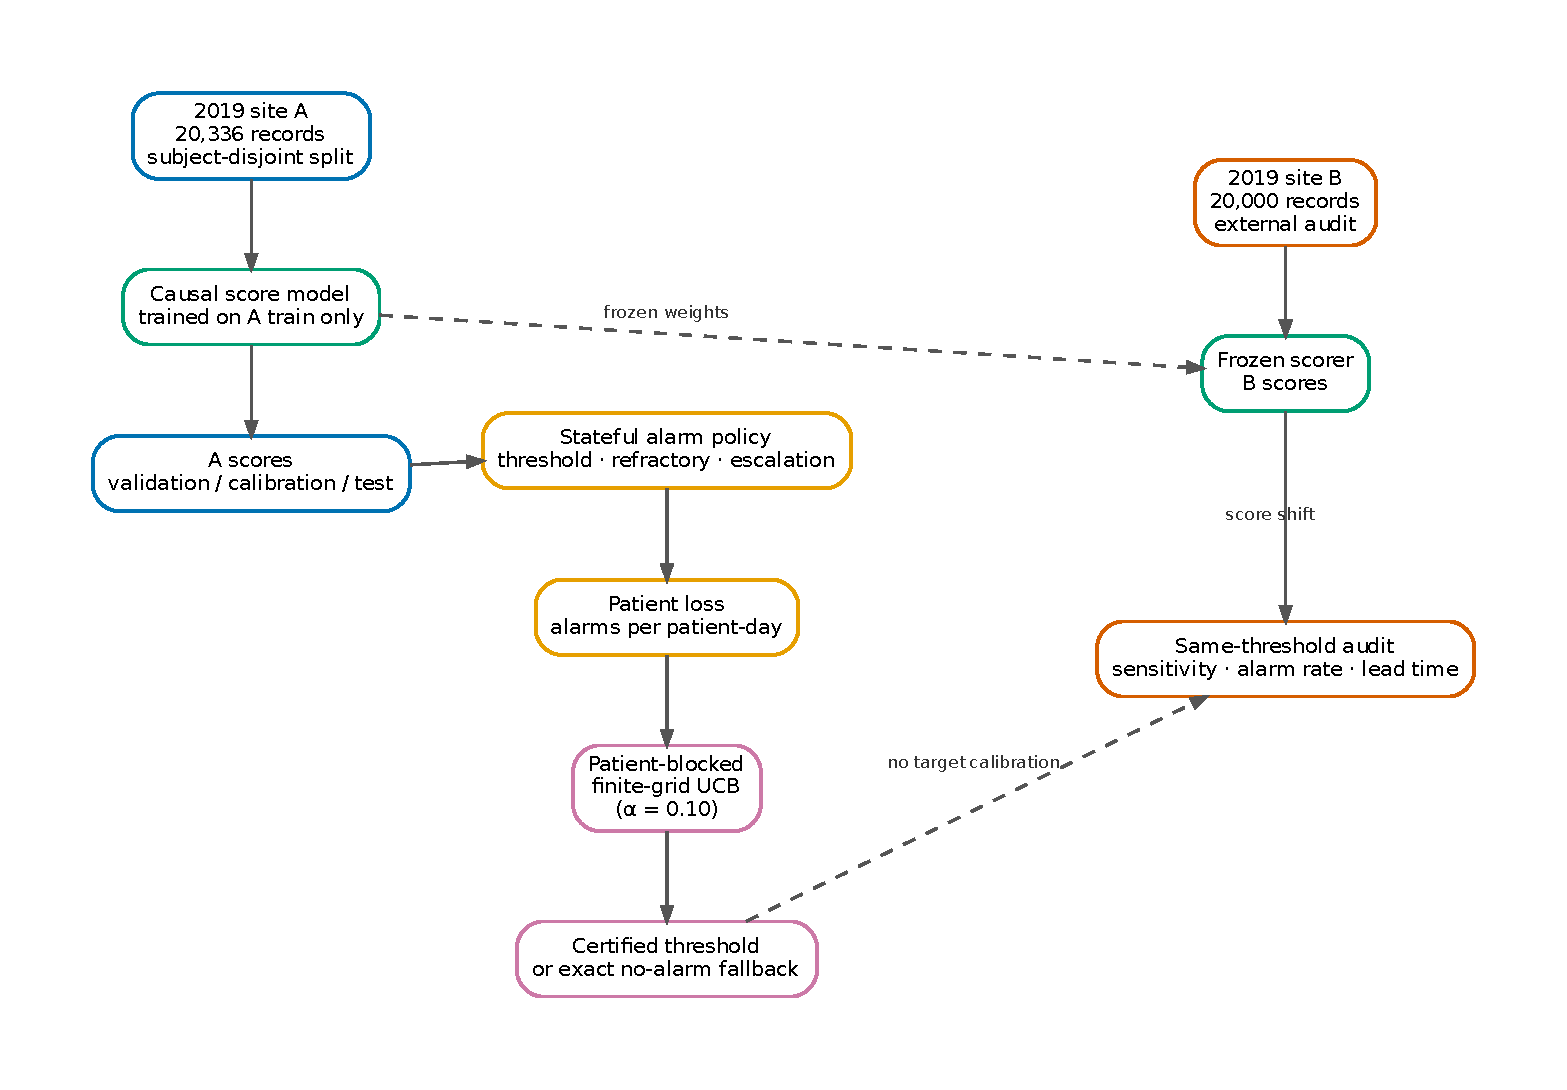
\includegraphics[width=\linewidth]{figures/framework.pdf}
\caption{Evaluation design. A causal score model is fitted on site A training records and frozen before site B is touched. The stateful policy replays each patient trajectory to obtain alarms per patient-day; a patient-blocked finite-grid upper confidence bound selects a threshold, or returns the exact no-alarm fallback when no candidate is certified. The primary external audit applies the same threshold without target-site calibration; the target-calibration diagnostic in the Results is a separate oracle analysis.}
\label{fig:framework}
\end{figure}

The audit also exposes substantial measurement heterogeneity. In site A, EtCO$_2$ is absent in every record, whereas 7.6\% of B records contain at least one EtCO$_2$ value; temperature is observed in only 33.8\% of A records, and several laboratory variables are observed in fewer than 5\%. This pattern motivates retaining a fixed variable set across sites and explicitly handling all-missing training columns, rather than fitting site-specific feature matrices. The 2012 mortality cohort \citep{citi2012physionet} was retained only as an ingestion and outcome-join check; because it has no deterioration onset, we do not treat its 49 decision points as a same-task external validation.

\subsection{Labels, Partitions and Eligibility}

The supplied 2019 label becomes positive six hours before the challenge-defined clinical onset. We set \texttt{label\_lead\_hours}$=6$ to recover the candidate clinical time and \texttt{horizon}$=6$ to label the six preceding hours positive. Timesteps at or after onset, padded steps, and all steps of a left-censored record are excluded from discrimination and calibration targets. An event at or beyond the end of observed follow-up is not counted as a detectable lead-time case.

The official 2019 release stores one PSV file per subject, and we use ``subject'' and ``patient'' interchangeably for this cohort. We use the file stem as the subject identifier and verify that every identifier occurs in exactly one partition; the split audit is written to the run metadata. For each random seed we use a subject-disjoint 60/15/10/15 split into training, validation, calibration and test subjects. The scorer, preprocessing, structural policy parameters and threshold grid are fixed using training and validation subjects. The calibration partition selects the deployed threshold, and the test partition is touched only for evaluation. Site B is evaluated with the A-trained scorer and the A-calibrated threshold; no B labels are used for target calibration. Three seeds (0, 1, 2) are reported for the prefix logistic model, the masked GRU, the LightGBM baseline and the E2 budget sweep. The target-site recalibration diagnostic is reported for all three logistic seeds and for one GRU seed, and is labelled as an oracle analysis throughout.

A separate target-site diagnostic asks how much of the external loss is recoverable when target labels are available. We split the eligible B subjects into disjoint calibration and test halves of equal size using a site-specific random permutation (seed $1000+s$ for source seed $s$), recalibrate the same policy family and threshold grid on B calibration subjects, and evaluate on B test subjects. This analysis uses target labels for threshold selection and is therefore an oracle-style target-calibrated reference estimate rather than a deployable label-free procedure; it is reported separately from the primary external audit and never used to tune the A model.

The target label-budget curve fixes the B test half and draws nested calibration subsets of 5\%, 10\%, 25\% and 50\% of all eligible B subjects from the remaining half. The same threshold selector is refitted on each subset and evaluated on the common test half, so the curve isolates calibration-set size. The source-threshold point is evaluated on the same test half and serves as the zero-label reference.

The support bound requires an independently declared minimum exposure. We use $H_{\min}=24$ hours, which retains 15{,}837 of 20{,}336 A records and 14{,}824 of 20{,}000 B records. This is an eligibility restriction, not a post-hoc filter chosen to improve results. Alarm-rate evaluation counts the full observed exposure, including time after onset; lead-time evaluation uses only the pre-onset window. With hourly decisions, refractory $\tau=4$ and no escalation, the resulting support bound is $L_{\max}=144/26\approx5.54$ alarms per patient-day.

\subsection{Score Models}

The primary scorer is a causal prefix-feature logistic regression. At each decision step it uses the last observed value of every variable, the cumulative observation fraction, and admission static features. All features are computed from current and past observations only. Median imputation is fitted on the training partition with empty features retained, so a variable that is entirely missing at site A remains a constant column at site B instead of silently changing the feature dimension. The classifier uses $C=1$ and a maximum of 2{,}000 iterations. A unidirectional masked GRU with 64 hidden units is used as a secondary architecture check. It consumes observed values, observation masks, log-transformed elapsed time and static features; it is a reference implementation, not a GRU-D reproduction. The GRU is trained for 20 epochs with Adam at $10^{-3}$, batch size 64, and a fixed random seed on an RTX 4090. A LightGBM gradient-boosted tree classifier is fitted to the same prefix features with 300 trees, learning rate 0.05, 31 leaves and median imputation; it is reported as a stronger tabular baseline, not as a tuned state-of-the-art model.

Partial NEWS, SIRS and qSOFA scores are computed from the variables available in the 2019 release, following the standard early-warning-score and instrument definitions \cite{price2023evaluating,candel2023development}. NEWS omits the consciousness and supplemental-oxygen components, SIRS omits the immature-neutrophil alternative, and qSOFA omits the Glasgow Coma Scale; these are research-only partial instruments, not certified clinical implementations. Charted observations are placed on the ICULOS clock, forward-filled, and scored per timestep. Steps before the first observed component are backfilled with the first finite score, and any remaining unobserved step receives zero points; this is a no-points convention, not an assertion that the patient was clinically normal. Their thresholds are calibrated on the same A calibration subjects at the same requested budgets as the learned scorers, so the comparison is a matched-workload audit rather than a claim that the instruments are equivalent.

\subsection{Alarm Policy and Calibration}

The policy family is the stateful rule in \cref{eq:policy}. We fix refractory $\tau=4$ decision steps, escalation $\kappa=0$, and a 12-hour lead window $W=12$. The candidate grid is 200 equally spaced thresholds from 0.01 to 0.99; the grid is fixed before calibration. The risk level is $\alpha=0.10$, and the reported certificates use the empirical-Bernstein radius in \cref{eq:bernstein}; Proposition~\ref{prop:eb} gives its finite-grid validity, while the Hoeffding radius in Proposition~\ref{prop:validity} is retained as the conservative variant. The selector deploys the smallest threshold whose raw empirical loss plus radius is at most the requested budget. If no threshold is certified, the exact no-alarm fallback is reported rather than silently substituting the largest finite threshold.

For each patient and threshold, the full stateful trajectory is replayed once to obtain alarms per patient-day. This loss matrix is reused across budgets and across the blocked and timestep procedures, so differences between procedures come only from the confidence radius and not from a different point estimator. The deliberately invalid timestep comparator substitutes calibration timesteps for calibration patients in the Hoeffding radius; it is a diagnostic, not a proposed method.

\subsection{Metrics and Uncertainty}

Discrimination is summarized by AUROC and AUPRC over usable pre-onset timesteps. Because the positive-timestep prevalence is only 1.27\% in the A test partition and 0.72\% at B, AUPRC is interpreted against that prevalence rather than against 0.5. Calibration is summarized by 10-bin expected calibration error (ECE); ECE is descriptive and does not establish clinical calibration. Operational metrics are the realised patient-average alarm rate, event sensitivity in the 12-hour lead window, median lead time among detected events, and the fraction of test patients whose per-day alarm count exceeds the requested budget.

Confidence intervals for score metrics use a patient-level bootstrap with 400 resamples, preserving within-patient dependence. Operational intervals use 2{,}000 patient-block resamples on seed 0 and resample whole target subjects, so within-subject alarm dependence is preserved; paired differences use the same resampled subjects and Holm correction across the reported comparisons. Two-sided bootstrap $p$-values are not a substitute for external validation. Operational curves report the mean and sample standard deviation over seeds; no interval is attached to the single-seed target-site GRU diagnostic.

\subsection{Reproducibility and Compute}

All raw records and score caches are kept outside the manuscript repository. The code exposes separate entry points for downloading and checksumming the 2019 release, auditing the official files, fitting and caching E1 scores, sweeping E2 budgets, bootstrap intervals and seed aggregation. The full test suite (135 tests) passes on the execution machine. The GRU uses CUDA but no formal GPU-hour or energy measurement was recorded; runtimes are therefore reported as implementation facts, not as a compute-efficiency claim.
